\subsection{The Harmony of the Spheres: When Astronomy Got Really Into Music Theory}

And so they developed what would become known as the \textbf{harmony of the spheres}: the idea that the planets orbited in perfect circles, spaced according to divine musical ratios. They couldn't hear this cosmic music, but they were convinced it was there (a kind of silent, celestial jazz).

To describe planetary motion, they began to craft early models using circles, spheres, and proportional distances. While not physically accurate, these models introduced the concept that mathematics could describe motion and structure beyond immediate human experience: a giant leap toward mathematical astronomy.

\begin{figure}[H]
   \centering
   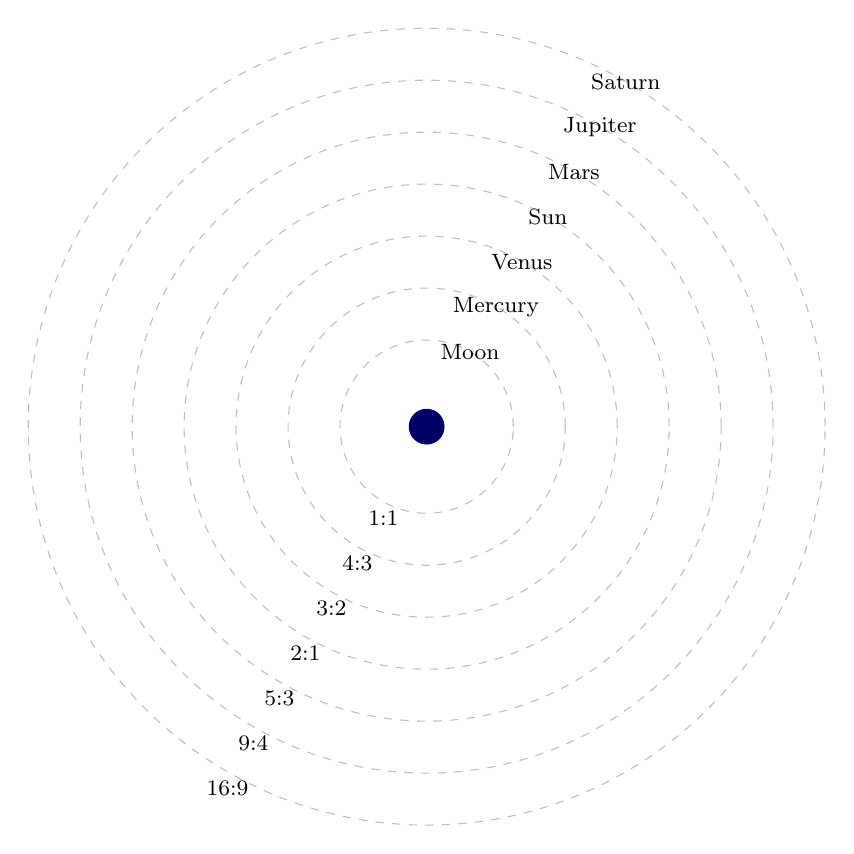
\begin{tikzpicture}[scale=2.2, every node/.style={font=\footnotesize}]
   
   % Central Earth
   %\filldraw[blue!40!black] (0,0) circle (0.1) node[white] {\textbf{Earth}};
   \filldraw[blue!40!black] (0,0) circle (0.1) node[white] {};
   
   % Radii, labels, and musical ratios
   \def\radii{{0.5, 0.8, 1.1, 1.4, 1.7, 2.0, 2.3}}
   \def\planets{{"Moon", "Mercury", "Venus", "Sun", "Mars", "Jupiter", "Saturn"}}
   \def\ratios{{"1:1", "4:3", "3:2", "2:1", "5:3", "9:4", "16:9"}}
   
   % Draw orbits and labels
   \foreach \r [count=\i] in {0.5, 0.8, 1.1, 1.4, 1.7, 2.0, 2.3} {
       \draw[gray!50, dashed] (0,0) circle (\r);
       \node at ({\r*cos(60)}, {\r*sin(60)}) {\pgfmathparse{\planets[\i-1]}\pgfmathresult};
       \node[below] at ({\r*cos(240)}, {\r*sin(240)}) {\pgfmathparse{\ratios[\i-1]}\pgfmathresult};
   }
   
   % Decorative arrows (hardcoded positions)
   %\draw[->, red!70] (0.5, 0) -- ++(0.2, 0.2);
   %\draw[->, red!70] (0.8, 0) -- ++(0.2, 0.15);
   %\draw[->, red!70] (1.1, 0) -- ++(0.2, 0.1);
   %\draw[->, red!70] (1.4, 0) -- ++(0.2, 0.05);
   %\draw[->, red!70] (1.7, 0) -- ++(0.2, 0);
   %\draw[->, red!70] (2.0, 0) -- ++(0.2, -0.05);
   %\draw[->, red!70] (2.3, 0) -- ++(0.2, -0.1);
   
   \end{tikzpicture}
   \caption{The \textbf{Harmony of the Spheres}: In Pythagorean cosmology, planetary orbits were spaced according to musical ratios. The Moon and Mercury were closest to Earth and produced low tones; Saturn was farthest, producing the highest tone in this cosmic scale.}
\end{figure}

\medskip

In short, the Pythagoreans turned proportion into a metaphysical framework. Where Egyptians used ratios to survive floods, the Greeks used them to explain the cosmos.

\medskip

\begin{tcolorbox}[colback=blue!5!white, colframe=blue!50!black, title={Historical Sidebar: Why Fantasy Worlds Feel Like the Harmony of the Spheres}]

    If you’re a fantasy nerd, the \textbf{Harmony of the Spheres} might sound strangely familiar. That’s because this ancient cosmology didn’t vanish: it quietly resurfaced in the works of modern mythmakers like \textbf{J.R.R. Tolkien} and \textbf{Brandon Sanderson}.

    \medskip
    
    Tolkien’s \textit{Silmarillion} opens with a creation story where the world is sung into existence by divine beings—the \textbf{Ainur}—under the guidance of a supreme composer. This isn’t just poetic license; it’s a direct echo of the Pythagorean belief that the cosmos was built on harmony, proportion, and celestial music. It’s a blend of Christian creation themes with the pagan idea that reality itself is structured like a grand, mathematical symphony.

    \medskip
    
    Meanwhile, Brandon Sanderson’s famous ``rules of magic'' --- logical, structured, and often tied to natural laws --- carry the philosophical fingerprints of Pythagorean thought. The idea that magic (or power) must operate within defined constraints and proportional systems is less about fantasy tropes and more about ancient metaphysics: the belief that unseen forces—whether gravity, music, or magic—obey rational, geometric principles.
    
    \medskip

    So when modern fantasy speaks of worlds governed by song, balance, or rigid magical laws, it’s not just world-building flair. It’s the \textbf{old cosmology} in disguise: a revival of the idea that the universe isn’t chaotic, but ordered, harmonious, and fundamentally mathematical.

    \medskip
    
    In other words, every time a wizard respects ``the balance,'' or a world is shaped by divine melodies, you’re hearing faint echoes of Pythagoras.
    
\end{tcolorbox}
